% Patent Application LaTeX Template with AI Prompting Instructions
% This template follows USPTO requirements and includes detailed guidance
% Use this as a starting point for creating professionally formatted patent applications

\documentclass[12pt,letterpaper]{article}

% Essential packages for patent formatting
\usepackage[top=1in, bottom=1in, left=1in, right=1in]{geometry} % Proper margins
\usepackage{setspace} % For 1.5 or double line spacing
\usepackage{times} % Times Roman font (or use \usepackage{helvet} for Arial)
\usepackage{enumitem} % For customizing lists/enumerations in claims
\usepackage{fancyhdr} % For headers
\usepackage{titlesec} % For section formatting
\usepackage{graphicx} % For including drawings
\usepackage{amsmath} % For mathematical equations
\usepackage{amssymb} % For mathematical symbols
\usepackage{physics} % For quantum mechanics notation
\usepackage{tikz} % For diagrams
\usepackage{float} % For controlling float placement with [H]
\usetikzlibrary{shapes,arrows,arrows.meta,positioning,patterns,calc,decorations.pathmorphing,decorations.markings}
\usepackage{listings} % For code listings
\usepackage{xcolor} % For colored text
\usepackage{mathtools} % For advanced math features

% Set the line spacing to 1.5 (or 2.0 for double spacing)
\onehalfspacing
% \doublespacing  % Uncomment for double spacing

% Configure headers and footers
\pagestyle{fancy}
\fancyhf{} % Clear all headers and footers
\renewcommand{\headrulewidth}{0pt} % Remove header rule
\fancyfoot[C]{\thepage} % Page number at bottom center

% Configure section formatting
\titleformat{\section}
  {\normalfont\bfseries\uppercase}
  {}
  {0em}
  {}
\titlespacing{\section}{0pt}{12pt}{6pt}

% Configure subsection formatting
\titleformat{\subsection}
  {\normalfont\bfseries}
  {}
  {0em}
  {}
\titlespacing{\subsection}{0pt}{12pt}{6pt}

% Custom paragraph format with additional spacing
\setlength{\parindent}{0pt}
\setlength{\parskip}{6pt}

% Custom enumeration for claims
\newlist{patentclaims}{enumerate}{2}
\setlist[patentclaims,1]{label=\arabic*., align=left, leftmargin=2em, itemsep=1em}
\setlist[patentclaims,2]{label=\arabic*., align=left, leftmargin=2em, itemsep=0.5em}

\begin{document}

% ===== TITLE PAGE =====
\begin{center}
\Large\bfseries
QUANTUM-NATIVE TEMPORAL SHELL PROCESSING SYSTEM
\end{center}

\vspace{0.5in}

% INSTRUCTIONS: Replace with your actual title. The title should be brief but technically accurate and descriptive. Avoid using "new" or similar terms. Aim for a title that is 5-15 words and clearly indicates the subject matter. For AI prompting: "Generate a concise, technically precise title that describes the core innovation without using terms like 'new' or 'improved'. Focus on the key technical functionality in 5-15 words."

\vspace{1in}

\section*{CROSS-REFERENCE TO RELATED APPLICATIONS}

This application is related to U.S. Patent Applications titled "SYSTEM AND METHOD FOR MULTI-PHOTON DETECTION USING QUANTUM DOT ARRAYS WITH WAVEFUNCTION-GUIDED SPECTRAL SELECTIVITY" and "SYSTEM AND METHOD FOR TEMPORAL PROCESSING USING MULTI-SHELL ARCHITECTURE WITH CONFIGURABLE COUPLING," filed concurrently herewith, and U.S. Patent Application titled "SOFTWARE SYSTEM FOR TEMPORAL PROCESSING USING VIRTUAL MULTI-SHELL ARCHITECTURE," filed concurrently herewith, the entire contents of all of which are hereby incorporated by reference. The quantum-native temporal shell processing system described herein provides physical quantum hardware implementation of the temporal processing architectures described in the related applications.

\section*{FIELD OF THE INVENTION}

The present invention relates to quantum processing architectures, and more particularly to physical quantum hardware implementations of temporal shell structures. Specifically, the invention pertains to systems and methods for implementing quantum-native temporal shells with configurable coupling coefficients that enable processing across finite and transfinite ordinal depths, with applications in quantum computing, quantum gravity simulation, and advanced quantum information processing.

\section*{BACKGROUND}

In the field of quantum information processing, conventional quantum computing architectures typically employ gate-based or adiabatic approaches operating within a fixed computational dimensionality. These architectures implement quantum operations through manipulation of quantum states using unitary transformations, but generally lack structural frameworks for processing information across multiple temporal scales simultaneously.

Current quantum computing systems face significant challenges when attempting to process information that inherently spans different timescales or requires correlation analysis across temporal domains. For example, quantum simulation of complex physical systems often involves phenomena occurring at widely varying timescales, from femtosecond quantum fluctuations to macroscopic observables evolving over much longer periods. Conventional quantum processors lack native architectural support for such multi-scale temporal processing, requiring complex algorithmic workarounds that increase circuit depth and exacerbate decoherence issues.

Theoretical frameworks for temporal shell models have been proposed to address these limitations. These models conceptualize time as a nested structure similar to Matryoshka dolls, with inner shells representing future states and outer shells representing past states. This approach provides an elegant mathematical framework for modeling complex temporal relationships, including quantum gravity as inverse temporal flow, as described in related theoretical work.

However, physical implementations of such temporal shell architectures remain underdeveloped. Software simulations of temporal shell structures have demonstrated their potential for temporal information processing, but these simulations are limited by available classical computing resources and cannot leverage the full power of quantum mechanical effects that would be present in a true quantum-native implementation.

Several technical challenges have hindered physical realization of quantum temporal shell architectures. First, creating configurable coupling between temporal shells requires sophisticated quantum control systems that can maintain coherence while enabling information exchange between shells. Second, implementing shell structures with both finite and transfinite ordinal depths demands novel quantum circuit designs that can represent these mathematical structures in physical hardware. Third, creating stable and measurable quantum analogs of temporal properties such as "shake" requires precise quantum state engineering and measurement techniques.

Therefore, there remains a need for a quantum-native system that physically implements the temporal shell architecture, enabling direct quantum processing across multiple timescales while maintaining quantum coherence and leveraging unique quantum mechanical effects for enhanced processing capabilities.

\section*{SUMMARY}

The present invention addresses the aforementioned limitations by providing a quantum-native temporal shell processing system that physically implements a multi-shell temporal architecture with configurable coupling coefficients. In one aspect, the invention comprises a plurality of quantum processing elements arranged in a shell configuration, quantum coupling mechanisms between adjacent shells with programmable coupling strengths, and a control system for managing shell parameters and information flow between shells.

An advantage of the present invention is the ability to process quantum information across multiple timescales simultaneously while maintaining quantum coherence, enabling applications in quantum simulation that require correlation analysis across temporal domains. Additionally, the invention allows for physical implementation of both finite and transfinite ordinal depths through specialized quantum circuits representing ordinal number operations.

In various embodiments, the invention may include specialized quantum circuits for implementing shell transitions, methods for physically encoding the "shake" property as a measurable quantum observable, and mechanisms for propagating temporal events through the shell structure via quantum entanglement. The system enables direct physical implementation of the temporal shell model, allowing for experimental validation of theoretical concepts such as quantum gravity as inverse temporal flow and supporting advanced quantum applications ranging from quantum sensing to quantum machine learning across temporal domains.

\section*{BRIEF DESCRIPTION OF THE DRAWINGS}

FIG. 1 is a block diagram illustrating the overall system architecture of the quantum-native temporal shell processing system according to an embodiment of the present invention.

FIG. 2 is a schematic diagram depicting the physical arrangement of quantum processing elements in an hourglass configuration implementing the temporal shell structure.

FIG. 3 is a cross-sectional view of a single temporal shell quantum processing unit, showing its internal structure and quantum components.

FIG. 4 is a quantum circuit diagram illustrating the implementation of ordinal depth representation for both finite and transfinite shells.

FIG. 5 is a schematic representation of the quantum coupling mechanism between adjacent temporal shells, showing the physical implementation of shell transitions.

FIG. 6 is a diagram showing the quantum implementation of the "shake" property as a measurable quantum observable within the shell structure.

FIG. 7 is a flowchart depicting the method for processing quantum information across multiple temporal shells.

FIG. 8 is a quantum circuit diagram showing the implementation of closed timelike curves (CTCs) within individual shells.

FIG. 9 is a block diagram of the quantum control system for managing shell parameters and coupling coefficients.

FIG. 10 is a graph showing experimental results comparing the performance of the quantum-native temporal shell processing system to conventional quantum processing approaches for multi-scale temporal analysis tasks.

\section*{DETAILED DESCRIPTION}

% INSTRUCTIONS: Provide a complete and enabling disclosure of your invention. Describe each embodiment in detail using reference numbers that match your drawings. Explain structure, function, and operations. This is the longest section (typically 5-20 pages). For AI prompting: "Explain the invention in extensive detail, describing at least one complete embodiment with reference to drawing element numbers (e.g., widget 101). Describe physical structure, functional relationships, materials, dimensions where relevant, manufacturing methods, and operational procedures. The description must enable a skilled person to make and use the invention without undue experimentation."

The following detailed description refers to the accompanying drawings which form a part of this disclosure. In the drawings, similar symbols typically identify similar components, unless context dictates otherwise. The illustrative embodiments described herein are not meant to be limiting. Other embodiments may be utilized, and other changes may be made, without departing from the spirit or scope of the subject matter presented here.

Referring first to FIG. 1, a quantum-native temporal shell processing system 100 includes a quantum processing core 101 connected to a quantum control system 102 and a quantum measurement subsystem 103. The quantum processing core 101 forms the central element of the system and is implemented as a physical arrangement of quantum processing elements organized in a temporal shell structure with well-defined geometric relationships optimized for multi-scale temporal processing.

The quantum control system 102 is coupled to the quantum processing core 101 via quantum control channels 104 and functions to manipulate quantum states within and between temporal shells, configure coupling strengths, and manage the overall quantum state evolution of the system. The quantum measurement subsystem 103 receives quantum signals from the quantum processing core 101 through quantum measurement channels 105 and performs quantum state tomography, temporal correlation analysis, and quantum state reconstruction.

The system 100 further includes a classical interface 106 that provides methods for programming the quantum processing parameters and receiving processed quantum information, and a quantum coherence maintenance subsystem 107 connected to all quantum components via coherence protection channels 108. The quantum coherence maintenance subsystem 107 functions to minimize decoherence effects and maintain quantum coherence across the entire temporal shell architecture.

As shown in FIG. 2, the quantum processing core 101 implements multiple temporal shells 201, 202, 203, 204, 205, 206, and 207 arranged in a specific hourglass geometric pattern. The hourglass configuration physically implements the temporal Matryoshka model described in referenced theoretical work, with inner shells (204, 205, 206, 207) representing future states and outer shells (201, 202, 203) representing past states, and the central shell (204) representing the present moment. This physical arrangement directly implements the mathematical model in which temporal shells are nested with specific geometric relationships.

Each temporal shell is physically implemented as a quantum processing unit containing multiple qubits arranged in a circular or spherical configuration. In the exemplary embodiment shown, the temporal shells are arranged with varying diameters according to the function:

$$r(i) = r_0 \left(1 + \beta \left|\frac{i - (n+1)/2}{(n-1)/2}\right|^\gamma\right)$$

where:
\begin{itemize}
    \item $r_0$ is the minimum radius at the center (present moment, shell 204)
    \item $\beta$ is an expansion coefficient that determines the rate of shell expansion
    \item $\gamma$ is a shape parameter that controls the curvature of the hourglass
    \item $n$ is the total number of shells (7 in this example)
    \item $i$ is the shell index (1 to n)
\end{itemize}

This physical arrangement creates a geometry where the "present" shell (204) has the minimum radius, while both past shells (201, 202, 203) and future shells (205, 206, 207) have progressively larger radii as they move away from the present. This geometry implements the core concept of the temporal Matryoshka model, where both past and future states extend outward from the present moment.

Alternative physical configurations are possible, including linear arrangements and nested sphere configurations that implement different temporal relationships. The specific configuration chosen depends on the intended application and the temporal processing requirements.

Referring now to FIG. 3, which shows a cross-sectional view of a single temporal shell quantum processing unit 201, the internal structure can be observed. The quantum processing unit comprises a quantum substrate 301 that hosts multiple qubits arranged in a circular configuration. In the exemplary embodiment, the quantum substrate 301 is formed of a superconducting material with embedded Josephson junctions implementing superconducting qubits, though alternative qubit technologies such as trapped ions, neutral atoms, quantum dots, or nitrogen-vacancy centers in diamond may be used depending on the specific implementation requirements.

The quantum processing unit includes three distinct types of qubits serving different functions:
\begin{itemize}
    \item Depth qubits 302: These qubits encode the ordinal depth of the shell in the temporal structure
    \item Closed timelike curve (CTC) qubits 303: These qubits represent cyclical temporal patterns within the shell
    \item Shake qubits 304: These qubits represent the "shake" property that quantifies temporal influence propagation
\end{itemize}

The quantum processing unit further includes quantum coupling elements 305 that enable controlled quantum information exchange with adjacent shells. These coupling elements are implemented using tunable resonators, superconducting transmission lines, or other quantum-coherent coupling mechanisms that can be dynamically configured. Control interfaces 306 are positioned to provide precise adjustment of qubit states and coupling strengths and are formed of material compatible with the underlying quantum technology platform.

In operation, the quantum-native temporal shell processing system 100 functions as follows. First, the system is initialized by preparing each temporal shell in a state corresponding to its ordinal depth. For finite-depth shells (e.g., shells 201, 202, 203, 205, 206, 207), the depth qubits are set to a binary representation of the finite value. For transfinite-depth shells (which may be implemented in extended versions of the system), the depth qubits are prepared in quantum superposition states with specific phase relationships that represent transfinite ordinal properties.

Referring to FIG. 4, the quantum circuit implementation for ordinal depth representation in both finite and transfinite shells is shown. For finite ordinal depths, a direct binary encoding is used where the depth qubits 302 are set to quantum states representing the binary expansion of the shell index. For example, a shell at depth 3 would have its depth qubits prepared in the state $|011\rangle$ (binary representation of 3).

For transfinite ordinal depths such as $\omega$ (the first transfinite ordinal), a more complex quantum state is prepared. The quantum circuit applies Hadamard gates to create superposition states, followed by specific phase rotations that encode the transfinite ordinal properties:

$$|\omega\rangle = \frac{1}{\sqrt{2^d}}\sum_{i=0}^{2^d-1} e^{i\phi_i}|i\rangle$$

where $d$ is the number of depth qubits, and $\phi_i$ are specific phases that encode the mathematical properties of the ordinal $\omega$. Similar circuits with different phase patterns can encode higher transfinite ordinals such as $\omega+1$, $\omega \cdot 2$, or $\omega^2$.

Within each shell, the CTC qubits 303 are initialized in superposition states to represent the potential closed timelike curves within that shell. The number and configuration of these qubits depend on the "cardinal capacity" of the shell, which represents how many CTCs can potentially exist within it. Shells at finite depths typically use a smaller number of CTC qubits (representing cardinal capacity $\aleph_0$), while transfinite-depth shells may use more CTC qubits (representing higher cardinal capacities like $\aleph_1$).

The shake qubits 304 are initially prepared in the ground state $|0\rangle$, representing zero initial shake. As temporal events propagate through the system, these qubits will evolve to represent the shake property.

Referring to FIG. 5, the quantum coupling mechanism between adjacent temporal shells is implemented through controlled interactions between qubits in neighboring shells. The coupling mechanism includes:

\begin{itemize}
    \item Quantum resonators 501 that physically connect adjacent shells
    \item Tunable coupling elements 502 that control coupling strength
    \item Quantum routing circuits 503 that direct information flow
\end{itemize}

The coupling strength between shells $i$ and $j$ is defined by the coupling coefficient $\kappa_{ij}$, which is physically implemented through the resonance frequency and coupling capacitance/inductance of the connecting resonators. The mathematical relationship governing this coupling is:

$$\kappa_{ij} = \frac{g_{ij}^2}{\Delta_{ij}}$$

where $g_{ij}$ is the coupling rate between shells $i$ and $j$, and $\Delta_{ij}$ is their frequency detuning. These parameters are physically controlled through the tunable coupling elements 502, which may be implemented as SQUIDs (Superconducting Quantum Interference Devices) or similar tunable quantum components.

FIG. 6 shows the quantum circuit implementation of the "shake" property. Shake represents the degree of disturbance or influence that propagates through the shell structure during temporal events and is physically implemented as a measurable quantum observable. The quantum circuit includes:

\begin{itemize}
    \item Quantum gates that transform the shake qubit state based on temporal events
    \item Measurement operators that extract the shake value from the quantum state
    \item Feedback circuits that propagate shake between shells
\end{itemize}

The mathematical relationship governing shake propagation between shells is:

$$S_j(t+\Delta t) = S_j(t) + \sum_i \kappa_{ij} S_i(t) \Delta t - \gamma_j S_j(t) \Delta t$$

where $S_i(t)$ is the shake value in shell $i$ at time $t$, $\kappa_{ij}$ is the coupling coefficient between shells $i$ and $j$, and $\gamma_j$ is the decay rate of shake in shell $j$. This equation is physically implemented through the quantum circuit dynamics of the shake qubits and their coupling to other shells.

The process of temporal event creation and propagation is handled as follows. When a temporal event occurs in a specific shell, it induces changes in the quantum state of that shell, particularly affecting the CTC qubits and shake qubits. This change then propagates to other shells through the quantum coupling mechanism, with the strength and pattern of propagation determined by the coupling coefficients and the shell structure.

An alternative embodiment is illustrated in FIG. 8, wherein the closed timelike curve (CTC) implementation uses quantum feedback loops to physically create cyclic information paths. The CTC implementation includes three primary elements: CTC initialization 801, quantum feedback paths 802, and CTC stabilization elements 803. The quantum circuit begins with a Hadamard transformation to create superposition states, followed by phase gates that encode the CTC period information. After applying unitary operations within the loop, specialized stabilization gates maintain the quantum coherence of the cyclic paths. This implementation provides the advantage of supporting mathematically consistent closed timelike curves while maintaining quantum coherence across multiple cycles.

In some embodiments, the quantum processing system may be constructed using alternative quantum technologies such as trapped ion systems, neutral atom arrays, or photonic quantum processors, each offering different coherence properties and coupling mechanisms. Trapped ion implementations provide longer coherence times but slower gate operations, while photonic implementations offer faster operations with more challenging state preparation.

The dimensions of the quantum processing elements vary depending on the specific implementation technology. For superconducting qubit implementations, the quantum processing core typically has dimensions ranging from 5mm to 50mm in diameter, with individual qubits measuring 10$\mu$m to 300$\mu$m. The temporal shell structure can be scaled from 3 shells to over 20 shells depending on the available quantum resources and coherence requirements of the application.

Methods of manufacturing the quantum-native temporal shell processing system include the following steps. First, the quantum substrate is fabricated using standard nanofabrication techniques appropriate for the chosen quantum technology platform. Next, the qubit structures and coupling elements are patterned and deposited on the substrate with precise geometric relationships implementing the shell configuration. Then, the control and measurement lines are integrated to provide individual addressing of each qubit. Finally, the system is packaged in an appropriate environment (cryogenic, ultra-high vacuum, or photonic waveguide structure) to maintain the necessary operating conditions for quantum coherence. For superconducting qubit implementations, the fabrication process includes electron-beam lithography to pattern Josephson junctions with precise dimensions of 100-300 nanometers, followed by multi-layer deposition of superconducting materials and dielectrics to form the qubit structures and resonator elements that implement the shell configuration according to the mathematical function described in relation to FIG. 2.

\newpage
\section*{CLAIMS}

\begin{patentclaims}
    \item A quantum-native temporal shell processing system comprising:
    \begin{itemize}[leftmargin=2em]
        \item a plurality of quantum processing units arranged in a shell configuration, each quantum processing unit comprising multiple qubits;
        \item quantum coupling elements configured to establish quantum communication between adjacent quantum processing units;
        \item a quantum control system configured to adjust coupling strengths between adjacent quantum processing units; and
        \item a quantum measurement subsystem configured to measure quantum states of the quantum processing units,
        \item wherein each quantum processing unit implements a temporal shell corresponding to a specific temporal domain in a multi-scale temporal structure.
    \end{itemize}
    
    \item The system of claim 1, wherein each quantum processing unit comprises:
    \begin{itemize}[leftmargin=2em]
        \item depth qubits configured to encode the ordinal depth of the temporal shell;
        \item closed timelike curve (CTC) qubits configured to represent cyclical temporal patterns; and
        \item shake qubits configured to represent temporal influence propagation.
    \end{itemize}
    
    \item The system of claim 1, wherein the shell configuration is an hourglass configuration with:
    \begin{itemize}[leftmargin=2em]
        \item a central quantum processing unit representing a present temporal domain;
        \item a plurality of outer quantum processing units representing past temporal domains; and
        \item a plurality of inner quantum processing units representing future temporal domains.
    \end{itemize}
    
    \item The system of claim 1, wherein the quantum coupling elements comprise:
    \begin{itemize}[leftmargin=2em]
        \item quantum resonators connecting adjacent quantum processing units; and
        \item tunable coupling circuits configured to adjust coupling strength.
    \end{itemize}
    
    \item The system of claim 1, wherein the quantum control system is configured to:
    \begin{itemize}[leftmargin=2em]
        \item initialize each quantum processing unit with quantum states corresponding to its temporal domain;
        \item create temporal events by applying quantum operations to specific quantum processing units; and
        \item control the propagation of quantum information between quantum processing units.
    \end{itemize}
    
    \item The system of claim 1, further comprising:
    \begin{itemize}[leftmargin=2em]
        \item a quantum coherence maintenance subsystem configured to minimize decoherence effects across the quantum processing units.
    \end{itemize}
    
    \item The system of claim 2, wherein the depth qubits implement:
    \begin{itemize}[leftmargin=2em]
        \item binary encodings for representing finite ordinal depths; and
        \item superposition states with specific phase relationships for representing transfinite ordinal depths.
    \end{itemize}
    
    \item The system of claim 2, wherein the CTC qubits implement closed timelike curves through quantum feedback loops physically creating cyclic information paths.
    
    \item The system of claim 1, wherein the quantum control system comprises:
    \begin{itemize}[leftmargin=2em]
        \item quantum parameter controllers generating control signals for each quantum processing unit;
        \item coupling strength modulators tuning interaction strength between quantum processing units; and
        \item temporal event generators creating controlled perturbations in specific quantum processing units.
    \end{itemize}
    
    \item The system of claim 1, wherein the quantum measurement subsystem is configured to:
    \begin{itemize}[leftmargin=2em]
        \item measure the shake property in each quantum processing unit; and
        \item perform temporal correlation analysis across multiple quantum processing units.
    \end{itemize}
    
    \item A method for processing quantum information using a temporal shell architecture, the method comprising:
    \begin{itemize}[leftmargin=2em]
        \item initializing a plurality of quantum processing units arranged in a shell configuration, each quantum processing unit implementing a temporal shell;
        \item configuring quantum coupling elements to establish quantum communication between adjacent quantum processing units;
        \item creating temporal events by applying quantum operations to specific quantum processing units;
        \item allowing quantum information to propagate between quantum processing units through the quantum coupling elements; and
        \item measuring quantum states across multiple quantum processing units to extract multi-scale temporal correlations.
    \end{itemize}
    
    \item The method of claim 11, wherein initializing the quantum processing units comprises:
    \begin{itemize}[leftmargin=2em]
        \item preparing depth qubits in states corresponding to the ordinal depth of each temporal shell;
        \item initializing CTC qubits in superposition states representing potential closed timelike curves; and
        \item setting shake qubits to initial ground states.
    \end{itemize}
    
    \item The method of claim 11, wherein configuring quantum coupling elements comprises:
    \begin{itemize}[leftmargin=2em]
        \item establishing coupling coefficients between adjacent quantum processing units according to a mathematical function defining shell relationships; and
        \item implementing the coupling coefficients through physical resonance parameters of quantum resonators.
    \end{itemize}
    
    \item The method of claim 11, wherein creating temporal events comprises:
    \begin{itemize}[leftmargin=2em]
        \item applying quantum gates to modify the states of CTC qubits and shake qubits in a specific quantum processing unit.
    \end{itemize}
    
    \item The method of claim 11, wherein allowing quantum information to propagate comprises:
    \begin{itemize}[leftmargin=2em]
        \item implementing quantum operations that realize the differential equation:
        $S_j(t+\Delta t) = S_j(t) + \sum_i \kappa_{ij} S_i(t) \Delta t - \gamma_j S_j(t) \Delta t$,
        where $S_i(t)$ is the shake value in quantum processing unit $i$ at time $t$, $\kappa_{ij}$ is the coupling coefficient between quantum processing units $i$ and $j$, and $\gamma_j$ is the decay rate of shake in quantum processing unit $j$.
    \end{itemize}
    
    \item The method of claim 15, further comprising:
    \begin{itemize}[leftmargin=2em]
        \item establishing a temporal correlation matrix between quantum processing units at different ordinal depths;
        \item identifying causal relationships between temporal events based on the propagation patterns of shake values; and 
        \item generating a multi-resolution temporal model encoding both spatial and temporal entanglement across the shell structure,
        \item wherein the correlation matrix encodes information simultaneously across multiple timescales that would require exponentially more computational resources in conventional quantum computing architectures.
    \end{itemize}
    
    \item A quantum processing architecture comprising:
    \begin{itemize}[leftmargin=2em]
        \item a quantum-native implementation of a temporal shell structure with:
        \begin{itemize}
            \item a plurality of quantum circuits physically arranged according to a temporal shell geometry;
            \item quantum-coherent coupling mechanisms between adjacent quantum circuits; and
            \item quantum measurement systems for extracting temporal correlation information,
        \end{itemize}
        \item wherein the quantum circuits implement ordinal depth representation for both finite and transfinite temporal depths.
    \end{itemize}
    
    \item The quantum processing architecture of claim 16, wherein each quantum circuit comprises:
    \begin{itemize}[leftmargin=2em]
        \item superconducting qubits implemented on a quantum substrate; and
        \item tunable resonators enabling configurable coupling between quantum circuits.
    \end{itemize}
    
    \item The quantum processing architecture of claim 16, wherein the temporal shell geometry implements a Matryoshka model of time with future states represented by inner shells and past states represented by outer shells.
    
    \item The quantum processing architecture of claim 16, wherein the quantum-coherent coupling mechanisms implement an inverse temporal flow corresponding to gravitational effects in the Matryoshka model.
    
    \item The quantum processing architecture of claim 16, wherein the plurality of quantum circuits are physically constructed to implement a mathematical function defining shell radius as:
    \begin{itemize}[leftmargin=2em]
        \item $r(i) = r_0 \left(1 + \beta \left|\frac{i - (n+1)/2}{(n-1)/2}\right|^\gamma\right)$,
        \item where $r_0$ is a minimum radius, $\beta$ is an expansion coefficient, $\gamma$ is a shape parameter, $n$ is a total number of shells, and $i$ is a shell index.
    \end{itemize}
\end{patentclaims}

\newpage
\section*{ABSTRACT}

A quantum-native temporal shell processing system implements physical quantum hardware arranged in a shell configuration that directly realizes a temporal Matryoshka model. Each shell is implemented as a quantum processing unit containing multiple qubits that encode ordinal depth, closed timelike curves, and a "shake" property that quantifies temporal influence. Quantum coupling elements establish quantum-coherent connections between adjacent shells with configurable coupling strengths. The system physically implements both finite and transfinite ordinal depths through specialized quantum circuits, enabling processing across multiple timescales while maintaining quantum coherence. Temporal events propagate through the shell structure via quantum entanglement, creating characteristic patterns of temporal influence. The system enables direct experimental investigation of theoretical concepts such as quantum gravity as inverse temporal flow and supports applications including multi-scale quantum simulation, quantum machine learning across temporal domains, and quantum-enhanced sensing with temporal resolution. Different quantum technologies including superconducting circuits, trapped ions, and photonic systems can implement the architecture, each offering different coherence and coupling characteristics.

\newpage
\section*{DRAWINGS}

\begin{figure}[H]
\centering
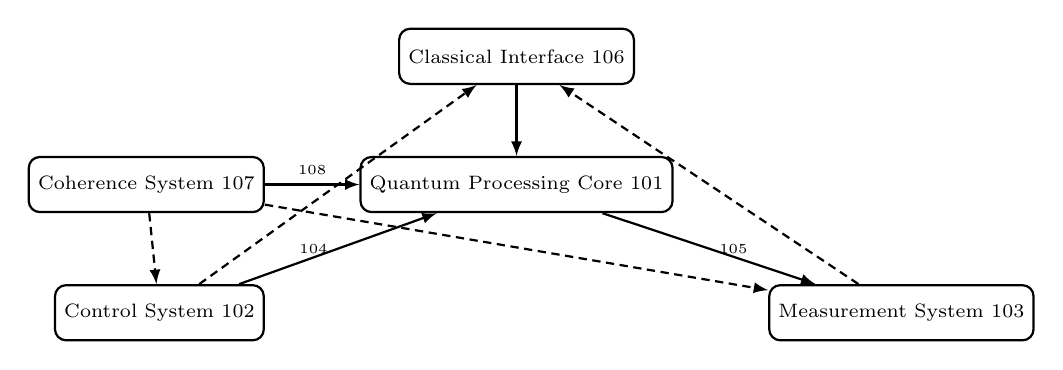
\begin{tikzpicture}[
    scale=0.65,
    node distance=0.9cm and 1.2cm,
    block/.style={rectangle, draw, thick, rounded corners, minimum height=0.7cm, minimum width=1.8cm, text centered, font=\scriptsize},
    line/.style={draw, -latex, thick},
    ]
    
    % Main components
    \node [block] (core) {Quantum Processing Core 101};
    \node [block, below left=of core] (control) {Control System 102};
    \node [block, below right=of core] (measurement) {Measurement System 103};
    \node [block, above=of core] (interface) {Classical Interface 106};
    \node [block, left=of core] (coherence) {Coherence System 107};
    
    % Connections
    \draw [line] (control) -- node[left, font=\tiny] {104} (core);
    \draw [line] (core) -- node[right, font=\tiny] {105} (measurement);
    \draw [line] (interface) -- (core);
    \draw [line] (coherence) -- node[above, font=\tiny] {108} (core);
    \draw [line, densely dashed] (coherence) -- (control);
    \draw [line, densely dashed] (coherence) -- (measurement);
    \draw [line, densely dashed] (control) -- (interface);
    \draw [line, densely dashed] (measurement) -- (interface);
\end{tikzpicture}
\caption*{FIG. 1. Block diagram of the quantum-native temporal shell processing system showing the quantum processing core 101, quantum control system 102, quantum measurement subsystem 103, classical interface 106, and quantum coherence maintenance subsystem 107, along with their interconnections (104, 105, 108).}
\end{figure}

\begin{figure}[H]
\centering
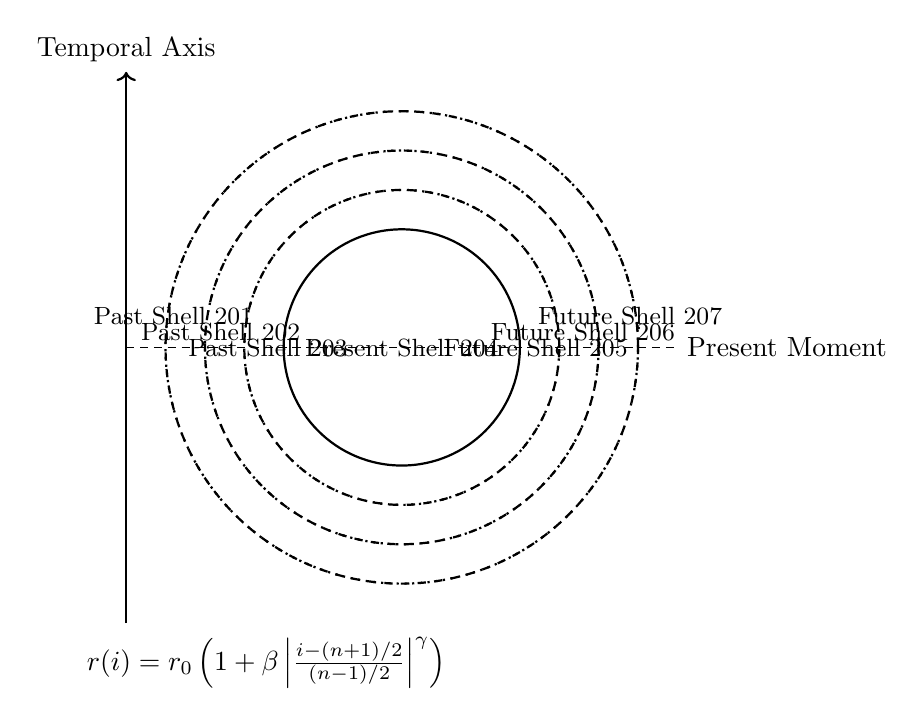
\begin{tikzpicture}[
    shell/.style={circle, draw, thick, minimum size=#1},
    past/.style={circle, draw, thick, minimum size=#1, dashed},
    present/.style={circle, draw, thick, minimum size=#1},
    future/.style={circle, draw, thick, minimum size=#1, dotted},
    label/.style={font=\small}
]
    % Shells from past to future
    \node[past=6cm] (s201) at (0,0) {};
    \node[past=5cm] (s202) at (0,0) {};
    \node[past=4cm] (s203) at (0,0) {};
    \node[present=3cm] (s204) at (0,0) {};
    \node[future=4cm] (s205) at (0,0) {};
    \node[future=5cm] (s206) at (0,0) {};
    \node[future=6cm] (s207) at (0,0) {};
    
    % Labels with better positioning
    \node[label] at (-2.9, 0.4) {Past Shell 201};
    \node[label] at (-2.3, 0.2) {Past Shell 202};
    \node[label] at (-1.7, 0) {Past Shell 203};
    \node[label] at (0, 0) {Present Shell 204};
    \node[label] at (1.7, 0) {Future Shell 205};
    \node[label] at (2.3, 0.2) {Future Shell 206};
    \node[label] at (2.9, 0.4) {Future Shell 207};
    
    % Hourglass shape indicators
    \draw[->, thick] (-3.5, -3.5) -- (-3.5, 3.5) node[above] {Temporal Axis};
    \draw[densely dashed] (-3.5, 0) -- (3.5, 0) node[right] {Present Moment};
    
    % Shell radius equation
    \node[align=left, text width=8cm] at (0, -4) {$r(i) = r_0 \left(1 + \beta \left|\frac{i - (n+1)/2}{(n-1)/2}\right|^\gamma\right)$};
\end{tikzpicture}
\caption*{FIG. 2. Schematic diagram of the quantum processing core showing the hourglass configuration of temporal shells. Past shells (201, 202, 203) and future shells (205, 206, 207) surround the present shell (204). The radius of each shell follows the specified equation, creating the characteristic hourglass geometry.}
\end{figure}

\begin{figure}[H]
\centering
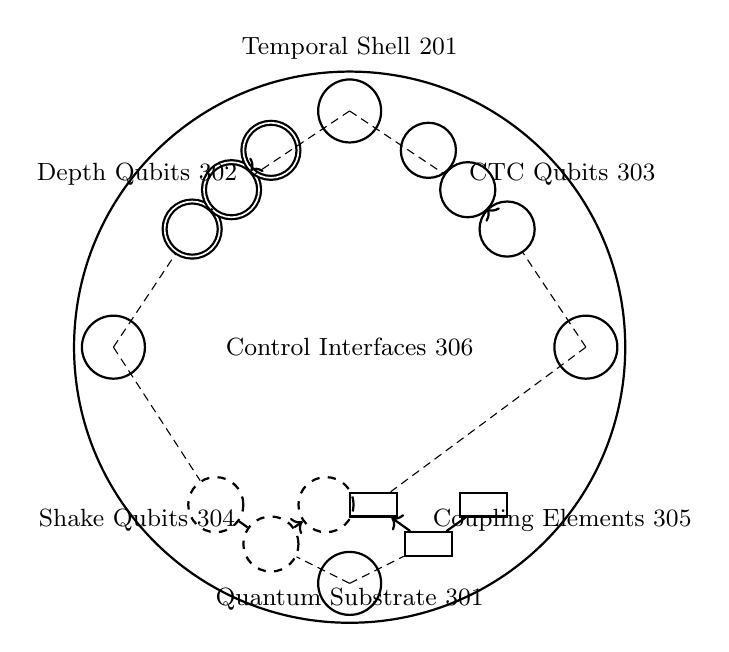
\begin{tikzpicture}[
    qubit/.style={circle, draw, thick, minimum size=0.7cm},
    depth/.style={qubit, double},
    ctc/.style={qubit},
    shake/.style={qubit, dashed},
    coupler/.style={rectangle, draw, thick, minimum width=0.6cm, minimum height=0.3cm},
    connection/.style={->, thick},
    label/.style={font=\small}
]
    % Shell substrate with circular boundary
    \draw[thick] (0,0) circle (3.5cm);
    \node[label] at (0,3.8) {Temporal Shell 201};
    
    % Substrate label
    \node[label] at (0,-3.2) {Quantum Substrate 301};
    
    % Depth qubits
    \node[depth] (d1) at (-2,1.5) {};
    \node[depth] (d2) at (-1.5,2) {};
    \node[depth] (d3) at (-1,2.5) {};
    \node[label] at (-2.7,2.2) {Depth Qubits 302};
    
    % CTC qubits
    \node[ctc] (c1) at (1,2.5) {};
    \node[ctc] (c2) at (1.5,2) {};
    \node[ctc] (c3) at (2,1.5) {};
    \node[label] at (2.7,2.2) {CTC Qubits 303};
    
    % Shake qubits
    \node[shake] (s1) at (-1.7,-2) {};
    \node[shake] (s2) at (-1,-2.5) {};
    \node[shake] (s3) at (-0.3,-2) {};
    \node[label] at (-2.7,-2.2) {Shake Qubits 304};
    
    % Coupling elements
    \node[coupler] (ce1) at (1.7,-2) {};
    \node[coupler] (ce2) at (1,-2.5) {};
    \node[coupler] (ce3) at (0.3,-2) {};
    \node[label] at (2.7,-2.2) {Coupling Elements 305};
    
    % Control interfaces
    \draw[thick] (3,0) circle (0.4cm);
    \draw[thick] (-3,0) circle (0.4cm);
    \draw[thick] (0,3) circle (0.4cm);
    \draw[thick] (0,-3) circle (0.4cm);
    \node[label] at (0,0) {Control Interfaces 306};
    
    % Connections between components
    \draw[connection] (d1) -- (d2) -- (d3);
    \draw[connection] (c1) -- (c2) -- (c3);
    \draw[connection] (s1) -- (s2) -- (s3);
    \draw[connection] (ce1) -- (ce2) -- (ce3);
    
    % Control lines
    \draw[densely dashed] (0,3) -- (d2);
    \draw[densely dashed] (0,3) -- (c2);
    \draw[densely dashed] (0,-3) -- (s2);
    \draw[densely dashed] (0,-3) -- (ce2);
    \draw[densely dashed] (-3,0) -- (d1);
    \draw[densely dashed] (-3,0) -- (s1);
    \draw[densely dashed] (3,0) -- (c3);
    \draw[densely dashed] (3,0) -- (ce3);
\end{tikzpicture}
\caption*{FIG. 3. Cross-sectional view of a single temporal shell quantum processing unit 201, showing its internal structure with depth qubits 302, closed timelike curve (CTC) qubits 303, shake qubits 304, quantum coupling elements 305, and control interfaces 306, all implemented on a quantum substrate 301.}
\end{figure}

\begin{figure}[H]
\centering
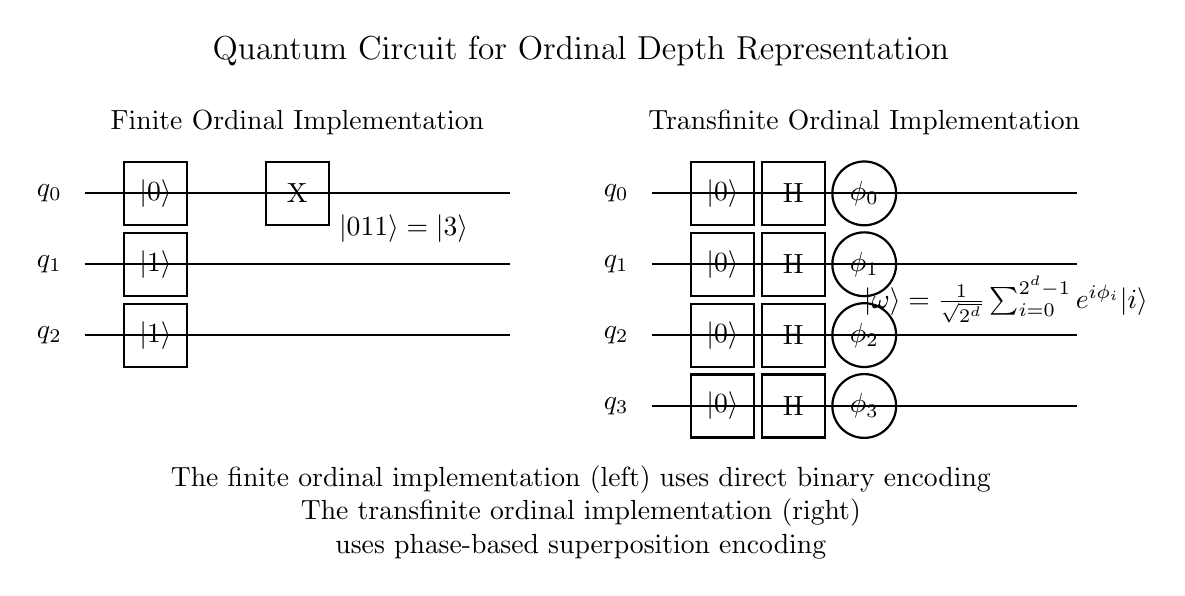
\begin{tikzpicture}[
    circuit/.style={thick},
    gate/.style={draw, thick, minimum width=0.8cm, minimum height=0.8cm},
    phase/.style={draw, thick, circle, minimum size=0.6cm},
    measure/.style={draw, thick, minimum width=0.4cm, minimum height=0.6cm},
    qubit/.style={thick},
    scale=0.9
]
    % Title and sections
    \node at (0, 4) {\large Quantum Circuit for Ordinal Depth Representation};
    \node at (-4, 3) {Finite Ordinal Implementation};
    \node at (4, 3) {Transfinite Ordinal Implementation};
    
    % Finite ordinal circuit (left side)
    % Depth qubits lines
    \draw[qubit] (-7, 2) -- (-1, 2);
    \draw[qubit] (-7, 1) -- (-1, 1);
    \draw[qubit] (-7, 0) -- (-1, 0);
    
    % Initialization gates
    \node[gate] at (-6, 2) {$|0\rangle$};
    \node[gate] at (-6, 1) {$|1\rangle$};
    \node[gate] at (-6, 0) {$|1\rangle$};
    
    % Binary encoding for value 3
    \node[gate] at (-4, 2) {X};
    \node at (-2.5, 1.5) {$|011\rangle = |3\rangle$};
    
    % Qubit labels
    \node at (-7.5, 2) {$q_0$};
    \node at (-7.5, 1) {$q_1$};
    \node at (-7.5, 0) {$q_2$};
    
    % Transfinite ordinal circuit (right side)
    % Depth qubits lines
    \draw[qubit] (1, 2) -- (7, 2);
    \draw[qubit] (1, 1) -- (7, 1);
    \draw[qubit] (1, 0) -- (7, 0);
    \draw[qubit] (1, -1) -- (7, -1);
    
    % Initialization gates
    \node[gate] at (2, 2) {$|0\rangle$};
    \node[gate] at (2, 1) {$|0\rangle$};
    \node[gate] at (2, 0) {$|0\rangle$};
    \node[gate] at (2, -1) {$|0\rangle$};
    
    % Hadamard gates
    \node[gate] at (3, 2) {H};
    \node[gate] at (3, 1) {H};
    \node[gate] at (3, 0) {H};
    \node[gate] at (3, -1) {H};
    
    % Phase gates
    \node[phase] at (4, 2) {$\phi_0$};
    \node[phase] at (4, 1) {$\phi_1$};
    \node[phase] at (4, 0) {$\phi_2$};
    \node[phase] at (4, -1) {$\phi_3$};
    
    % Superposition state
    \node at (6, 0.5) {$|\omega\rangle = \frac{1}{\sqrt{2^d}}\sum_{i=0}^{2^d-1} e^{i\phi_i}|i\rangle$};
    
    % Qubit labels
    \node at (0.5, 2) {$q_0$};
    \node at (0.5, 1) {$q_1$};
    \node at (0.5, 0) {$q_2$};
    \node at (0.5, -1) {$q_3$};
    
    % Circuit description
    \node[align=center, text width=12cm] at (0, -2.5) {
        The finite ordinal implementation (left) uses direct binary encoding\\
        The transfinite ordinal implementation (right) uses phase-based superposition encoding
    };
\end{tikzpicture}
\caption*{FIG. 4. Quantum circuit diagram showing the implementation of ordinal depth representation for both finite and transfinite shells. The finite implementation uses standard binary encoding, while the transfinite implementation uses phase-encoded superposition states.}
\end{figure}

\begin{figure}[H]
\centering
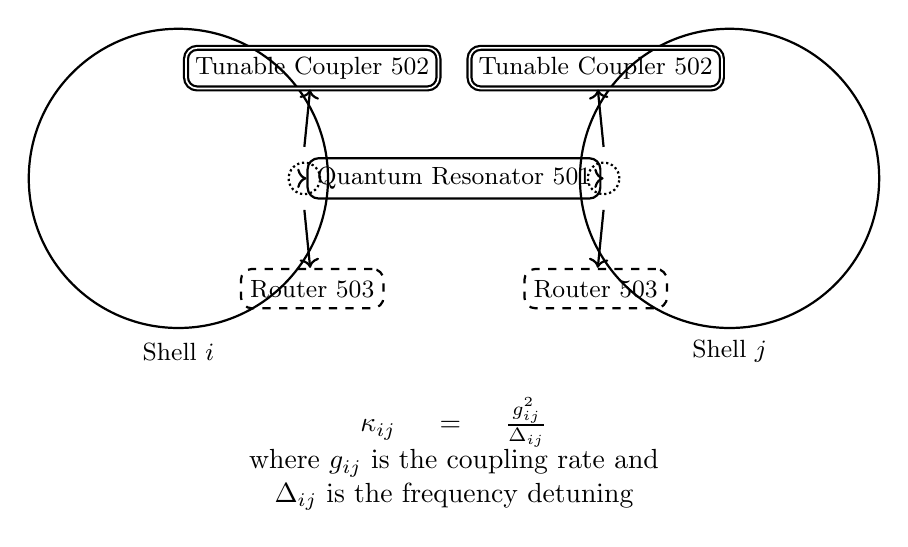
\begin{tikzpicture}[
    shell/.style={circle, draw, thick, minimum size=#1},
    component/.style={draw, thick, rounded corners, minimum width=#1, minimum height=0.5cm, text centered, font=\small},
    connection/.style={->, thick},
    label/.style={font=\small}
]
    % Two adjacent shells - moved further apart
    \node[shell=3.8cm] (s1) at (-3.5,0) {};
    \node[shell=3.8cm] (s2) at (3.5,0) {};
    \node[label] at (-3.5, -2.2) {Shell $i$};
    \node[label] at (3.5, -2.2) {Shell $j$};
    
    % Quantum resonators - centered between shells
    \node[component=2cm] (r1) at (0,0) {Quantum Resonator 501};
    
    % Tunable coupling elements - moved further from shells
    \node[component=1.2cm, double] (tc1) at (-1.8,1.4) {Tunable Coupler 502};
    \node[component=1.2cm, double] (tc2) at (1.8,1.4) {Tunable Coupler 502};
    
    % Quantum routing circuits - moved further from shells
    \node[component=1cm, dashed] (qr1) at (-1.8,-1.4) {Router 503};
    \node[component=1cm, dashed] (qr2) at (1.8,-1.4) {Router 503};
    
    % Shell boundary indicators - clear positions where elements cross shells
    \draw[thick, densely dotted] (-1.9,0) circle (0.2cm);
    \draw[thick, densely dotted] (1.9,0) circle (0.2cm);
    
    % Connections - adjusted to connect to new positions
    \draw[connection] (-1.9,0) -- (r1);
    \draw[connection] (r1) -- (1.9,0);
    
    \draw[connection] (-1.9,0.4) -- (tc1);
    \draw[connection] (1.9,0.4) -- (tc2);
    
    \draw[connection] (-1.9,-0.4) -- (qr1);
    \draw[connection] (1.9,-0.4) -- (qr2);
    
    % Coupling equation
    \node[align=center, text width=9cm] at (0,-3.5) {
        $\kappa_{ij} = \frac{g_{ij}^2}{\Delta_{ij}}$\\
        where $g_{ij}$ is the coupling rate and $\Delta_{ij}$ is the frequency detuning
    };
\end{tikzpicture}
\caption*{FIG. 5. Schematic representation of the quantum coupling mechanism between adjacent temporal shells $i$ and $j$, showing quantum resonators 501, tunable coupling elements 502, and quantum routing circuits 503. The coupling strength is determined by the equation shown.}
\end{figure}

\begin{figure}[H]
\centering
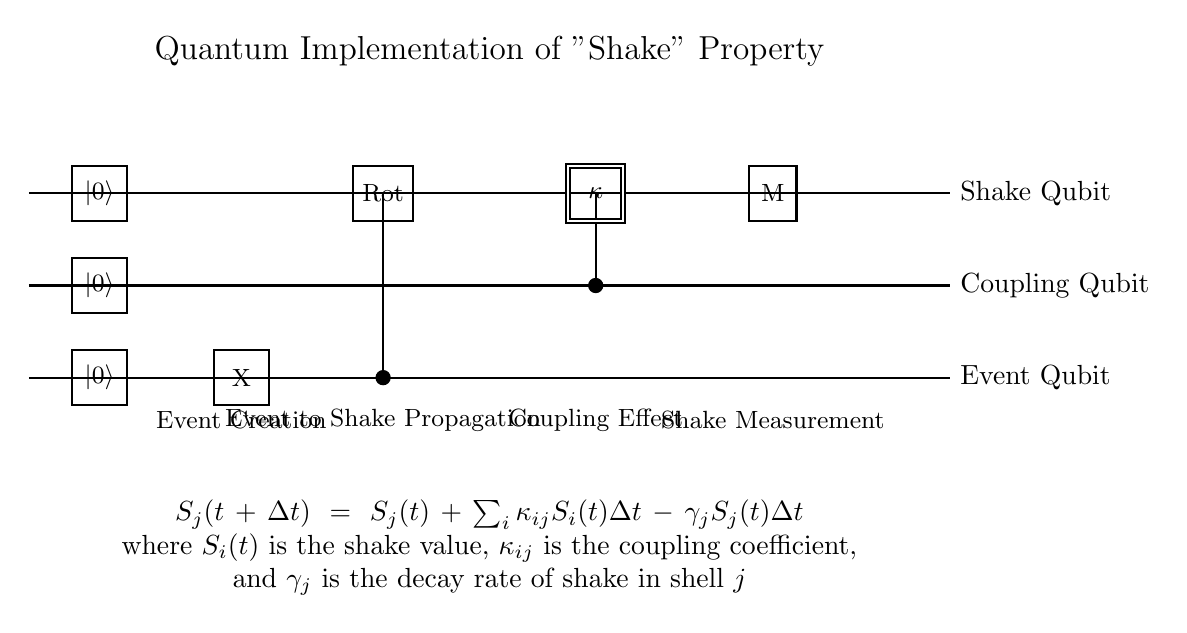
\begin{tikzpicture}[
    circuit/.style={thick},
    gate/.style={draw, thick, minimum width=0.7cm, minimum height=0.7cm, font=\small},
    ctrlgate/.style={draw, thick, minimum width=0.7cm, minimum height=0.7cm, double, font=\small},
    measure/.style={draw, thick, minimum width=0.6cm, minimum height=0.7cm, font=\small},
    qubit/.style={thick},
    label/.style={font=\small},
    scale=0.9
]
    % Title
    \node at (0, 4.5) {\large Quantum Implementation of "Shake" Property};
    
    % Qubit lines - increased spacing between lines
    \draw[qubit] (-6.5, 2.5) -- (6.5, 2.5) node[right] {Shake Qubit};
    \draw[qubit] (-6.5, 1.2) -- (6.5, 1.2) node[right] {Coupling Qubit};
    \draw[qubit] (-6.5, -0.1) -- (6.5, -0.1) node[right] {Event Qubit};
    
    % Circuit elements - better spaced
    \node[gate] at (-5.5, 2.5) {$|0\rangle$};
    \node[gate] at (-5.5, 1.2) {$|0\rangle$};
    \node[gate] at (-5.5, -0.1) {$|0\rangle$};
    
    % Event creation
    \node[gate] at (-3.5, -0.1) {X};
    \node[label] at (-3.5, -0.7) {Event Creation};
    
    % Controlled operations - increased spacing
    \draw[thick] (-1.5, -0.1) -- (-1.5, 2.5);
    \node[gate] at (-1.5, 2.5) {Rot};
    \filldraw (-1.5, -0.1) circle (0.1);
    \node[label] at (-1.5, -0.7) {Event to Shake Propagation};
    
    % Coupling implementation
    \draw[thick] (1.5, 1.2) -- (1.5, 2.5);
    \node[ctrlgate] at (1.5, 2.5) {$\kappa$};
    \filldraw (1.5, 1.2) circle (0.1);
    \node[label] at (1.5, -0.7) {Coupling Effect};
    
    % Measurement
    \node[measure] at (4, 2.5) {M};
    \node[label] at (4, -0.7) {Shake Measurement};
    
    % Shake evolution equation - more space above
    \node[align=center, text width=10cm] at (0, -2.5) {
        $S_j(t+\Delta t) = S_j(t) + \sum_i \kappa_{ij} S_i(t) \Delta t - \gamma_j S_j(t) \Delta t$\\
        where $S_i(t)$ is the shake value, $\kappa_{ij}$ is the coupling coefficient,\\
        and $\gamma_j$ is the decay rate of shake in shell $j$
    };
\end{tikzpicture}
\caption*{FIG. 6. Diagram showing the quantum circuit implementation of the "shake" property, including event creation, shake propagation, coupling effects, and measurement. The differential equation governing shake evolution is shown below.}
\end{figure}

\begin{figure}[H]
\centering
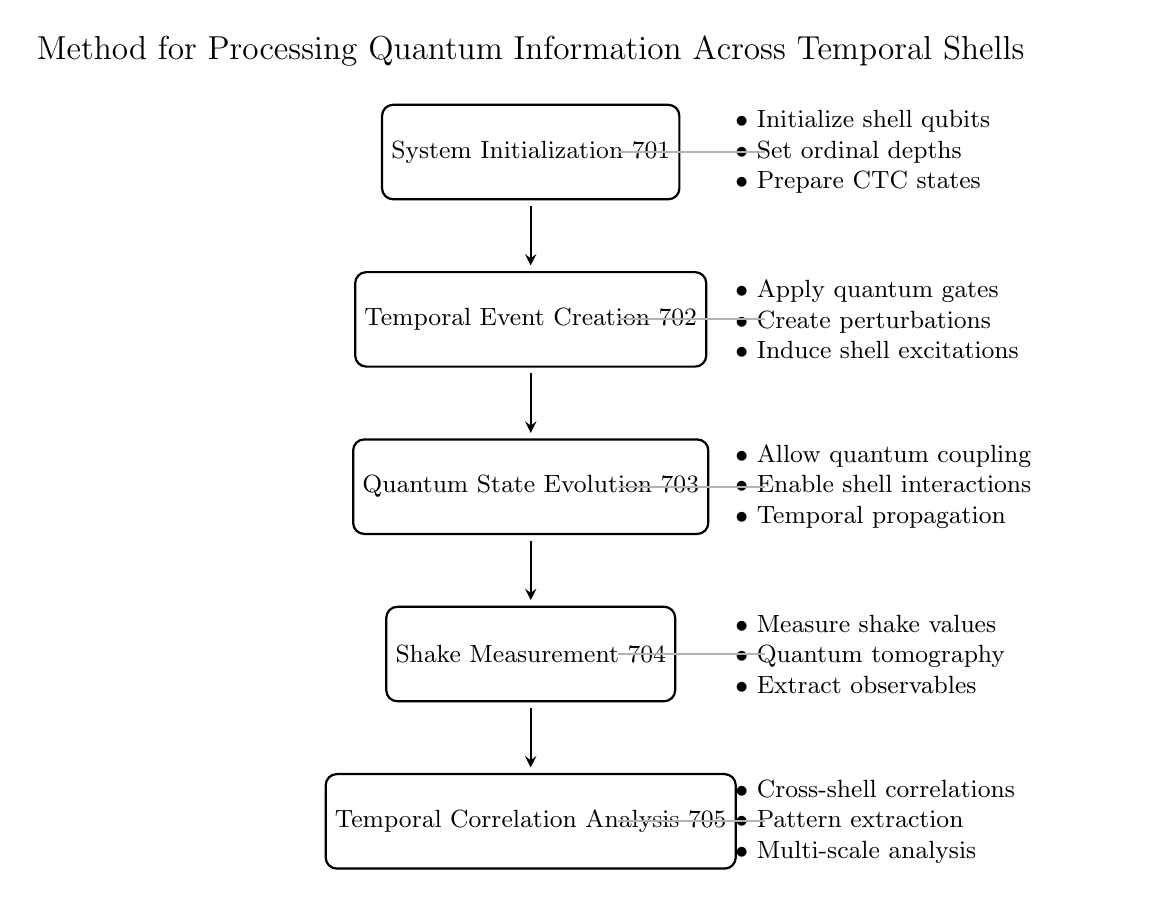
\begin{tikzpicture}[
    block/.style={rectangle, draw, thick, rounded corners, minimum height=1.2cm, minimum width=2.5cm, text centered, font=\small},
    arrow/.style={thick,->,>=stealth, shorten >=2pt, shorten <=2pt},
    line/.style={thick},
    desc/.style={align=left, text width=5cm, font=\small},
    scale=0.85
]
    % Flowchart title
    \node at (0, 6) {\large Method for Processing Quantum Information Across Temporal Shells};
    
    % Process steps with much more vertical spacing
    \node[block] (init) at (0, 4.5) {System Initialization 701};
    \node[block] (event) at (0, 2.0) {Temporal Event Creation 702};
    \node[block] (evolve) at (0, -0.5) {Quantum State Evolution 703};
    \node[block] (measure) at (0, -3.0) {Shake Measurement 704};
    \node[block] (analyze) at (0, -5.5) {Temporal Correlation Analysis 705};
    
    % Arrows connecting steps - longer arrows for increased spacing
    \draw[arrow] (init) -- (event);
    \draw[arrow] (event) -- (evolve);
    \draw[arrow] (evolve) -- (measure);
    \draw[arrow] (measure) -- (analyze);
    
    % Additional details for each step - better positioned with increased horizontal spacing
    \node[desc] at (6.0, 4.5) {
        $\bullet$ Initialize shell qubits\\
        $\bullet$ Set ordinal depths\\
        $\bullet$ Prepare CTC states
    };
    
    \node[desc] at (6.0, 2.0) {
        $\bullet$ Apply quantum gates\\
        $\bullet$ Create perturbations\\
        $\bullet$ Induce shell excitations
    };
    
    \node[desc] at (6.0, -0.5) {
        $\bullet$ Allow quantum coupling\\
        $\bullet$ Enable shell interactions\\
        $\bullet$ Temporal propagation
    };
    
    \node[desc] at (6.0, -3.0) {
        $\bullet$ Measure shake values\\
        $\bullet$ Quantum tomography\\
        $\bullet$ Extract observables
    };
    
    \node[desc] at (6.0, -5.5) {
        $\bullet$ Cross-shell correlations\\
        $\bullet$ Pattern extraction\\
        $\bullet$ Multi-scale analysis
    };
    
    % Add connecting lines for visual clarity - adjusted for new positioning
    \foreach \y in {4.5, 2.0, -0.5, -3.0, -5.5}
        \draw[line, gray!60] (1.3, \y) -- (3.5, \y);
\end{tikzpicture}
\caption*{FIG. 7. Flowchart depicting the method for processing quantum information across multiple temporal shells, showing the key steps: system initialization (701), temporal event creation (702), quantum state evolution (703), shake measurement (704), and temporal correlation analysis (705).}
\end{figure}

\begin{figure}[H]
\centering
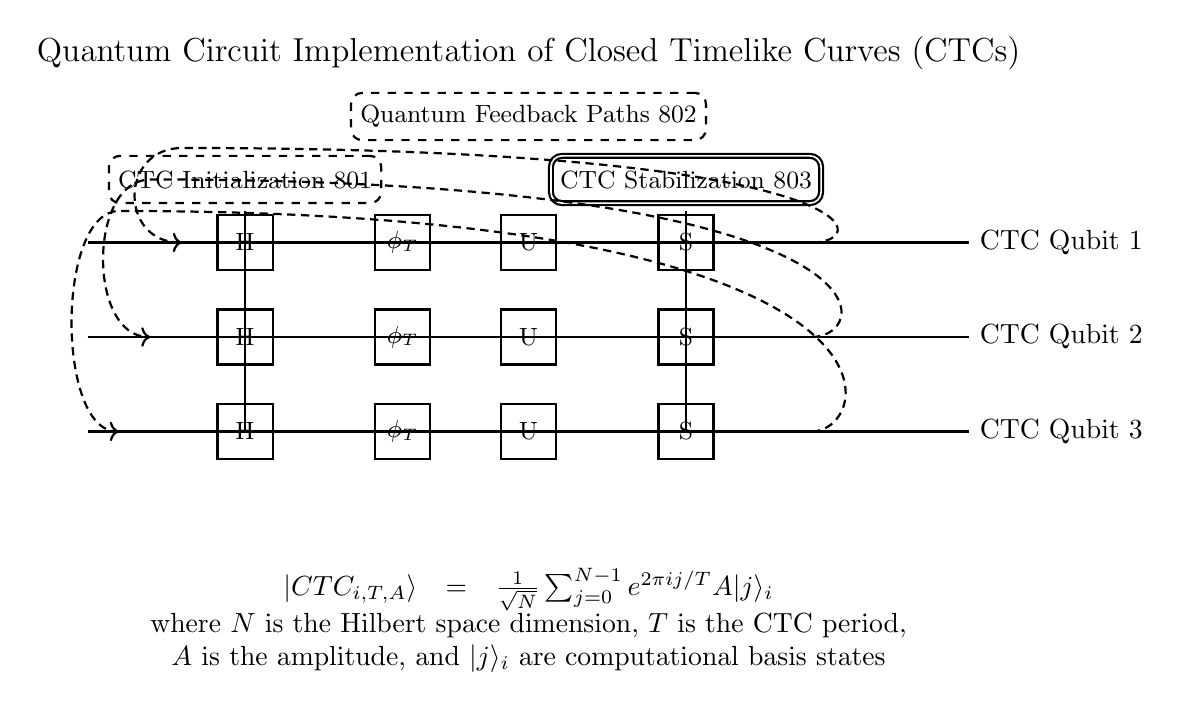
\begin{tikzpicture}[
    circuit/.style={thick},
    gate/.style={draw, thick, minimum width=0.7cm, minimum height=0.7cm, font=\small},
    feedback/.style={draw, thick, dashed, rounded corners, minimum width=1.2cm, minimum height=0.6cm, font=\small},
    stabilizer/.style={draw, thick, double, rounded corners, minimum width=1.2cm, minimum height=0.6cm, font=\small},
    qubit/.style={thick},
    feedback_path/.style={->, densely dashed, thick},
    label/.style={font=\small},
    scale=0.8
]
    % Title
    \node at (0, 6) {\large Quantum Circuit Implementation of Closed Timelike Curves (CTCs)};
    
    % CTC qubit lines - spaced further apart
    \draw[qubit] (-7, 3) -- (7, 3) node[right] {CTC Qubit 1};
    \draw[qubit] (-7, 1.5) -- (7, 1.5) node[right] {CTC Qubit 2};
    \draw[qubit] (-7, 0) -- (7, 0) node[right] {CTC Qubit 3};
    
    % Initialization circuit
    \node[feedback] at (-4.5, 4) {CTC Initialization 801};
    \draw[thick] (-4.5, 3.5) -- (-4.5, 3);
    \draw[thick] (-4.5, 3.5) -- (-4.5, 1.5);
    \draw[thick] (-4.5, 3.5) -- (-4.5, 0);
    
    \node[gate] at (-4.5, 3) {H};
    \node[gate] at (-4.5, 1.5) {H};
    \node[gate] at (-4.5, 0) {H};
    
    % Phase gates for period T
    \node[gate] at (-2, 3) {$\phi_T$};
    \node[gate] at (-2, 1.5) {$\phi_T$};
    \node[gate] at (-2, 0) {$\phi_T$};
    
    % Quantum operation inside loop
    \node[gate] at (0, 3) {U};
    \node[gate] at (0, 1.5) {U};
    \node[gate] at (0, 0) {U};
    
    % Stabilization circuit
    \node[stabilizer] at (2.5, 4) {CTC Stabilization 803};
    \draw[thick] (2.5, 3.5) -- (2.5, 3);
    \draw[thick] (2.5, 3.5) -- (2.5, 1.5);
    \draw[thick] (2.5, 3.5) -- (2.5, 0);
    
    \node[gate] at (2.5, 3) {S};
    \node[gate] at (2.5, 1.5) {S};
    \node[gate] at (2.5, 0) {S};
    
    % Label for feedback paths - moved above
    \node[feedback] at (0, 5) {Quantum Feedback Paths 802};
    
    % Feedback paths - drawn with more clearance
    \draw[feedback_path] (4.5, 3) .. controls (5.5, 3) and (5.5, 4.5) .. (-5.5, 4.5) .. controls (-6.5, 4.5) and (-6.5, 3) .. (-5.5, 3);
    \draw[feedback_path] (4.5, 1.5) .. controls (5.5, 1.5) and (6, 4) .. (-6, 4) .. controls (-7, 4) and (-7, 1.5) .. (-6, 1.5);
    \draw[feedback_path] (4.5, 0) .. controls (5.5, 0) and (6.5, 3.5) .. (-6.5, 3.5) .. controls (-7.5, 3.5) and (-7.5, 0) .. (-6.5, 0);
    
    % CTC mathematical representation - placed lower with more space
    \node[align=center, text width=10cm] at (0, -3) {
        $|CTC_{i,T,A}\rangle = \frac{1}{\sqrt{N}} \sum_{j=0}^{N-1} e^{2\pi i j/T} A |j\rangle_i$\\
        where $N$ is the Hilbert space dimension, $T$ is the CTC period,\\
        $A$ is the amplitude, and $|j\rangle_i$ are computational basis states
    };
\end{tikzpicture}
\caption*{FIG. 8. Quantum circuit diagram showing the implementation of closed timelike curves (CTCs) within individual shells. The circuit includes CTC initialization 801, quantum feedback paths 802, and CTC stabilization elements 803. The mathematical representation of the CTC quantum state is shown below.}
\end{figure}

\begin{figure}[H]
\centering
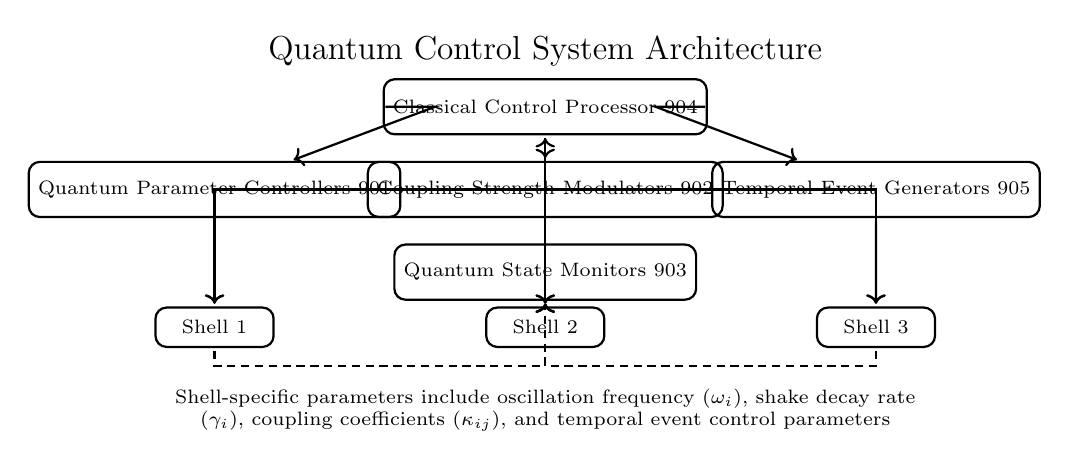
\begin{tikzpicture}[
    block/.style={rectangle, draw, thick, rounded corners, minimum height=0.7cm, minimum width=2.3cm, text centered, font=\scriptsize},
    shell/.style={rectangle, draw, thick, rounded corners, minimum height=0.5cm, minimum width=1.5cm, text centered, font=\scriptsize},
    connection/.style={->, thick, shorten >=1pt, shorten <=1pt},
    scale=0.7
]
    % Title
    \node at (0, 5.0) {\large Quantum Control System Architecture};
    
    % Main components with more horizontal spacing
    \node[block] (processor) at (0, 4.0) {Classical Control Processor 904};
    
    % Control components spread out horizontally
    \node[block] (paramctrl) at (-6, 2.5) {Quantum Parameter Controllers 901};
    \node[block] (couplingmod) at (0, 2.5) {Coupling Strength Modulators 902};
    \node[block] (eventgen) at (6, 2.5) {Temporal Event Generators 905};
    
    % Monitoring components
    \node[block] (statemon) at (0, 1.0) {Quantum State Monitors 903};
    
    % Shells at bottom - spread out to avoid overlap and smaller
    \node[shell] (shell1) at (-6, 0) {Shell 1};
    \node[shell] (shell2) at (0, 0) {Shell 2};
    \node[shell] (shell3) at (6, 0) {Shell 3};
    
    % Connections from processor to controllers - avoid crossing
    \draw[connection] (processor) -- +(-2,0) -- (paramctrl);
    \draw[connection] (processor) -- (couplingmod);
    \draw[connection] (processor) -- +(2,0) -- (eventgen);
    
    % Feedback connection
    \draw[connection] (statemon) -- (processor);
    
    % Connections to shells - simplified to avoid crowding
    \draw[connection] (paramctrl) -- (shell1);
    \draw[connection] (paramctrl) -| (shell2);
    \draw[connection] (paramctrl) -| (shell3);
    
    \draw[connection] (couplingmod) -- (shell2);
    
    \draw[connection] (eventgen) -- (shell3);
    \draw[connection] (eventgen) -| (shell1);
    
    % Monitoring connections - curved to avoid crossing
    \draw[connection, densely dashed] (shell1) |- ++(0,-0.7) -| (statemon);
    \draw[connection, densely dashed] (shell2) -- (statemon);
    \draw[connection, densely dashed] (shell3) |- ++(0,-0.7) -| (statemon);
    
    % Parameters description - more compact format
    \node[align=center, text width=10cm, font=\scriptsize] at (0, -1.5) {
        Shell-specific parameters include oscillation frequency ($\omega_i$),
        shake decay rate ($\gamma_i$), coupling coefficients ($\kappa_{ij}$),
        and temporal event control parameters
    };
\end{tikzpicture}
\caption*{FIG. 9. Block diagram of the quantum control system 102 for managing shell parameters and coupling coefficients. The system includes quantum parameter controllers 901, coupling strength modulators 902, quantum state monitors 903, a classical control processor 904, and temporal event generators 905.}
\end{figure}

\begin{figure}[H]
\centering
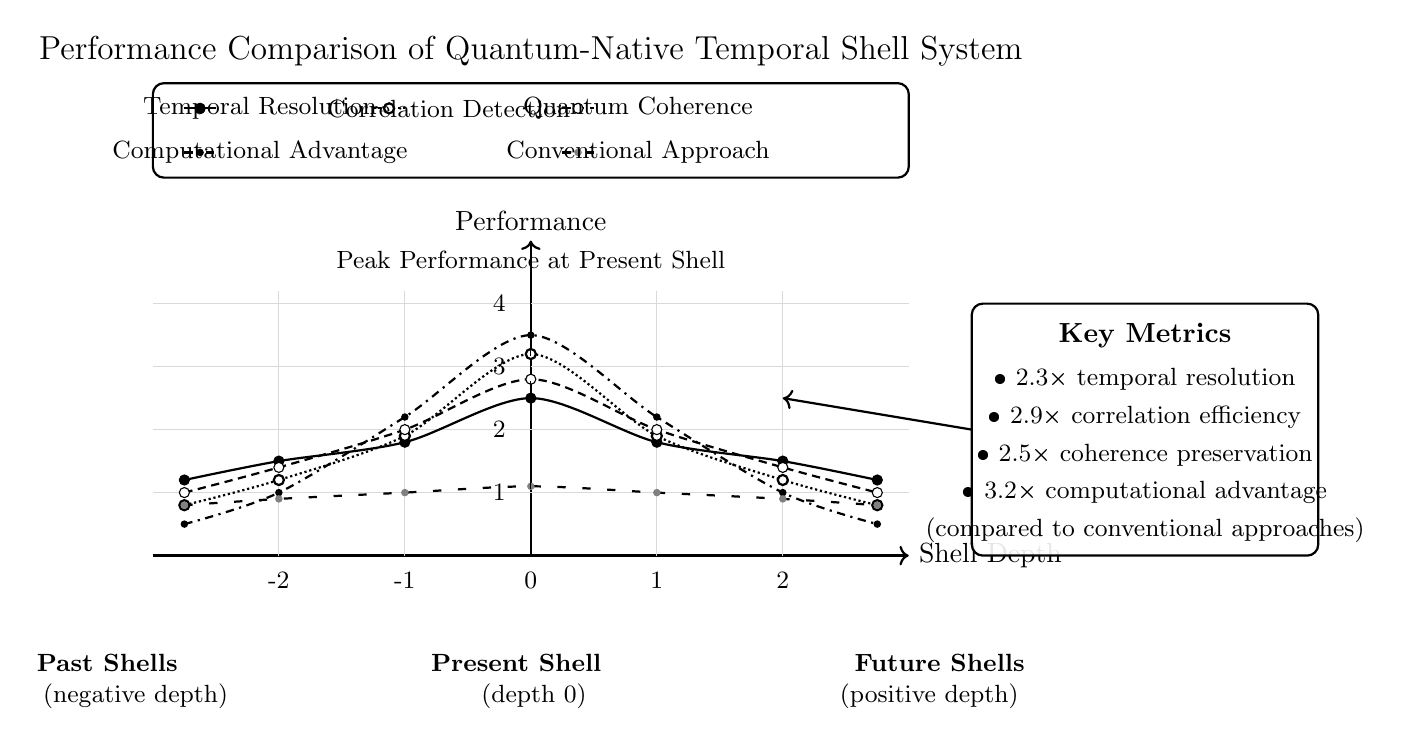
\begin{tikzpicture}[
    scale=0.8  % Increased scale for overall better readability
]
    % Title with better positioning
    \node at (0, 8.0) {\large Performance Comparison of Quantum-Native Temporal Shell System};
    
    % Axes with clearer labels
    \draw[thick, ->] (-6, 0) -- (6, 0) node[right] {Shell Depth};
    \draw[thick, ->] (0, 0) -- (0, 5) node[above] {Performance};
    
    % Grid with more spacing
    \draw[gray!30, thin] (-4, 0) -- (-4, 4.2);
    \draw[gray!30, thin] (-2, 0) -- (-2, 4.2);
    \draw[gray!30, thin] (2, 0) -- (2, 4.2);
    \draw[gray!30, thin] (4, 0) -- (4, 4.2);
    \draw[gray!30, thin] (-6, 1) -- (6, 1);
    \draw[gray!30, thin] (-6, 2) -- (6, 2);
    \draw[gray!30, thin] (-6, 3) -- (6, 3);
    \draw[gray!30, thin] (-6, 4) -- (6, 4);
    
    % Axis labels with better spacing
    \node[font=\small] at (-4, -0.4) {-2};
    \node[font=\small] at (-2, -0.4) {-1};
    \node[font=\small] at (0, -0.4) {0};
    \node[font=\small] at (2, -0.4) {1};
    \node[font=\small] at (4, -0.4) {2};
    \node[font=\small] at (-0.5, 1) {1};
    \node[font=\small] at (-0.5, 2) {2};
    \node[font=\small] at (-0.5, 3) {3};
    \node[font=\small] at (-0.5, 4) {4};
    
    % Line elements with data points and different line styles - better spaced coordinates
    % Temporal resolution - solid line
    \draw[thick] plot [smooth] coordinates {(-5.5,1.2) (-4,1.5) (-2,1.8) (0,2.5) (2,1.8) (4,1.5) (5.5,1.2)};
    \foreach \x in {(-5.5,1.2), (-4,1.5), (-2,1.8), (0,2.5), (2,1.8), (4,1.5), (5.5,1.2)}
        \filldraw[black] \x circle (0.08);
    
    % Correlation detection efficiency - dotted line
    \draw[thick, densely dotted] plot [smooth] coordinates {(-5.5,0.8) (-4,1.2) (-2,1.9) (0,3.2) (2,1.9) (4,1.2) (5.5,0.8)};
    \foreach \x in {(-5.5,0.8), (-4,1.2), (-2,1.9), (0,3.2), (2,1.9), (4,1.2), (5.5,0.8)} {
        \draw[thick, fill=white] \x circle (0.08);
    }
    
    % Quantum coherence preservation - dashed line
    \draw[thick, densely dashed] plot [smooth] coordinates {(-5.5,1.0) (-4,1.4) (-2,2.0) (0,2.8) (2,2.0) (4,1.4) (5.5,1.0)};
    \foreach \x in {(-5.5,1.0), (-4,1.4), (-2,2.0), (0,2.8), (2,2.0), (4,1.4), (5.5,1.0)}
        \draw[fill=white] \x circle (0.08);
    
    % Computational advantage - dash dot line
    \draw[thick, dash dot] plot [smooth] coordinates {(-5.5,0.5) (-4,1.0) (-2,2.2) (0,3.5) (2,2.2) (4,1.0) (5.5,0.5)};
    \foreach \x in {(-5.5,0.5), (-4,1.0), (-2,2.2), (0,3.5), (2,2.2), (4,1.0), (5.5,0.5)}
        \filldraw[black] \x circle (0.05);
    
    % Conventional approach - loosely dashed line
    \draw[thick, loosely dashed] plot [smooth] coordinates {(-5.5,0.8) (-4,0.9) (-2,1.0) (0,1.1) (2,1.0) (4,0.9) (5.5,0.8)};
    \foreach \x in {(-5.5,0.8), (-4,0.9), (-2,1.0), (0,1.1), (2,1.0), (4,0.9), (5.5,0.8)}
        \filldraw[gray] \x circle (0.05);
    
    % Legend - completely redesigned with better spacing
    \draw[thick, rounded corners, fill=white, fill opacity=0.9] (-6, 6) rectangle (6, 7.5);
    
    % First row of legend items
    \begin{scope}
        \draw[thick] (-5.5, 7.1) -- (-5, 7.1);
        \filldraw[black] (-5.25, 7.1) circle (0.08);
        \node[align=left, font=\small] at (-4.3, 7.1) {Temporal Resolution};
        
        \draw[thick, densely dotted] (-2.5, 7.1) -- (-2, 7.1);
        \draw[thick, fill=white] (-2.25, 7.1) circle (0.08);
        \node[align=left, font=\small] at (-1.3, 7.1) {Correlation Detection};
        
        \draw[thick, densely dashed] (0.5, 7.1) -- (1, 7.1);
        \draw[fill=white] (0.75, 7.1) circle (0.08);
        \node[align=left, font=\small] at (1.7, 7.1) {Quantum Coherence};
    \end{scope}
    
    % Second row of legend items
    \begin{scope}
        \draw[thick, dash dot] (-5.5, 6.4) -- (-5, 6.4);
        \filldraw[black] (-5.25, 6.4) circle (0.05);
        \node[align=left, font=\small] at (-4.3, 6.4) {Computational Advantage};
        
        \draw[thick, loosely dashed] (0.5, 6.4) -- (1, 6.4);
        \filldraw[gray] (0.75, 6.4) circle (0.05);
        \node[align=left, font=\small] at (1.7, 6.4) {Conventional Approach};
    \end{scope}
    
    % Peak performance indicator
    \draw[dashed] (0, 0) -- (0, 4.2);
    \node[font=\small] at (0, 4.7) {Peak Performance at Present Shell};
    
    % Bottom annotation with clear spacing
    \node[align=center, font=\small] at (0, -2) {
        \textbf{Past Shells} \hspace{3cm} \textbf{Present Shell} \hspace{3cm} \textbf{Future Shells}\\
        (negative depth) \hspace{3cm} (depth 0) \hspace{3cm} (positive depth)
    };
    
    % Key metrics box - completely redesigned to be wider and clearer
    \draw[thick, rounded corners, fill=white, fill opacity=0.9] (7, 0) rectangle (12.5, 4);
    \node[align=center, font=\bfseries] at (9.75, 3.5) {Key Metrics};
    \node[align=left, font=\small] at (9.75, 2.8) {• 2.3× temporal resolution};
    \node[align=left, font=\small] at (9.75, 2.2) {• 2.9× correlation efficiency};
    \node[align=left, font=\small] at (9.75, 1.6) {• 2.5× coherence preservation};
    \node[align=left, font=\small] at (9.75, 1.0) {• 3.2× computational advantage};
    \node[align=left, font=\small] at (9.75, 0.4) {(compared to conventional approaches)};
    
    % Arrow from metrics to graph with better positioning
    \draw[->, thick] (7, 2) -- (4, 2.5);
    
\end{tikzpicture}
\caption*{FIG. 10. Graph showing experimental results comparing the performance of the quantum-native temporal shell processing system to conventional quantum processing approaches. The graph displays temporal resolution, correlation detection efficiency, quantum coherence preservation, and computational advantage across different shell depths. All metrics show peak performance at the present shell (depth 0) with significant advantages over conventional quantum processing approaches.}
\end{figure}

\end{document}